\section{Application: App/OS Behavior}
\label{sec:characterize-app}

Privacy has rapidly become a critical issue for networked services, as large numbers of organizations develop 
extensive tracking infrastructure to gather information from users for ads and analytics. While the problem 
is well known and has been extensively studied in previous work~\cite{roesner:webtrackers,leontiadis:mobileads,vallina-rod:ads}, in this section we explore the potential to 
identify personals identifiable information (PII) exclusively from passively gathered app traces. Our key 
contributions are 1) we conduct controlled experiments to identify how PII is being leaked by apps via 
their network flows and 2) use SSL bumping enabled by \platname{} to understand how this information is being shared over 
secure channels (in addition to those revealed in the clear). 
For our analysis we focus on {\it what} PII is sent,  {\it to whom} is the PII sent, and {\it how frequently} is PII sent.
%To answer these questions, we rely on the controlled experiments and the \mobWild dataset.

We evaluate PII in terms of two threat models. First, we assume a passive eavesdropper that can sniff 
traffic over open WiFi APs or within a cellular provider. Any PII sent unencrypted is available to the attacker. 
Second, we assume an attack conducted by (or on) a third-party service that is able to identify a user's fine-grained locations 
over time. 

\begin{table*}[t]    
    \centering
    \begin{small}
    \begin{tabular}{|l|l|l|l|l|l|l|l|l|l|}
       \hline
       {\bf Store}&{\bf Platform}&{\bf \# Apps}&{\bf Email}& {\bf Location}& {\bf Name} &{\bf Password}& {\bf Device ID}& {\bf Contacts}& {\bf IMEI}\\
       \hline
       App Store&iPhone&209&13 (6.2\%) &20 (9.5\%)&4 (1.9\%)&6 (2.87\%)&4 (1.9\%)&0 (0\%)&0 (0\%)\\
       \hline
       Google Play&Android&100&3 (3\%)&10 (10\%)&2 (2\%)&1 (1\%)&21 (21\%)&0 (0\%)&13 (13\%)\\
       \hline
       Third Party&Android&908&1 (0.1\%)&32 (3.5\%)&2 (0.2\%)&0 (0\%)&95 (10.4\%)&4 (0.4\%)&48 (5.3\%)\\
       \hline
    \end{tabular}
    \end{small}
    \caption{Summary of personally identifiable information leaked in plaintext (HTTP) by Android and iPhone apps. \emph{The popular iOS apps tend to leak the location information in the clear while Android apps leak the IMEI number and Android ID in the clear.}}
    \label{tab:pii}
\end{table*}

\subsection{Controlled experiments}

For our experiments, we created fake user accounts with fake contact
information, and fake Twitter and Facebook accounts.  Our goal is to
detect if any PII---email
address, phone number, IMEI number---stored on the device is leaked
across the network over HTTP or HTTPS (using the SSL bumping plugin).
Some of this information is required for normal app operation; however, we strongly believe that such information should
never travel across the network in plaintext (HTTP). 

In Table~\ref{tab:pii}, we present the different PII leaked by both Android and iPhone apps.  We observe that
the IMEI, a unique identifier tied to a phone, is the most commonly
leaked PII by Android apps.  This IMEI can be used to track
and correlate a user's behavior across Web services.  Similarly, we
observe that Android apps leak the Android ID, a unique
identifier tied to an Android device.  In Table~\ref{tab:pii}, we also
observe that other information like contacts, emails, and passwords
are leaked in the clear.  The email address, the address used to sign
up for the services, was leaked in the clear by 13 iOS and 3 Android
apps from our set of popular apps.

While only one Android app (belonging to the \emph{Photography} category) leaked a password in the clear, 
we were surprised to learn that six of the most popular iOS apps send user 
credentials in the clear, \emph{including the password}. Particularly disconcerting 
is our observation that an app in the Medicine category -- which the provider claims has ``\emph{1 million active members 
of which 50\% are US physicians}'' -- sends the user's first name, last name, 
email, password, and zip code in the clear. Given US physician access to highly sensitive 
data like medical records, we believe it is particularly important for this app to protect 
user credentials (which are often used for multiple services). 

% For your eyes only ;)
%services.epocrates.com  Mozilla/5.0 (iPhone; U; CPU iPhone OS 4_0 like Mac OS X; en-us) AppleWebKit/532.9 (KHTML, like Gecko) Version/4.0.5 Mobile/8A293 Safari/6531.22.7   1370172894.1735 JXMXaFcr2Pd 10.11.4.52  55904   63.241.66.139   80  7   GET /userprofile/userprofile/userprofile/userprofile?datatype=json&os=6.1.3&device_model=iPhone&appVersion=5.2&appId=nc-2&data={"countryId":"10","lastName":"Test","firstName":"Meddle","password":"epocratespwdW1","passwordConfirm":"epocratespwdW1","email":"mailmeddle@yahoo.com","occupationId":"56","zipCode":"98105"}&action=useraccount&platform=14&subaction=createuser    -   0   40001   200 OK  -   -   -   (empty) -   -   -   text/plain  -   -   -   0       -   -   shen

\begin{table}
    \centering
    \begin{small}
    \begin{tabular}{|l|c|c||c|}
       \hline
       {\bf Host}&{\bf IMEI}&{\bf Device ID} & {\em Ads \& Analytics} \tabularnewline
       \hline              
       chartboost.com                & \checkmark & \checkmark & \checkmark  \tabularnewline
       tapjoyads.com                 & \checkmark & -          & \checkmark  \tabularnewline
       getjar.com                    & \checkmark & \checkmark & -   \tabularnewline
       pocketchange.com              & \checkmark & \checkmark & -   \tabularnewline
       iheart.com                    & \checkmark & \checkmark & -   \tabularnewline
       aarki.net                     & \checkmark & -          & \checkmark  \tabularnewline
       zynga.com                     & \checkmark & -          & -   \tabularnewline
       droidsecurity.appspot.com     & \checkmark & -          & -   \tabularnewline
       google.com                    & -          & \checkmark & -   \tabularnewline
       flurry.com                    & -          & \checkmark & \checkmark  \tabularnewline
       groupon.com                   & -          & \checkmark & -   \tabularnewline
       \hline
    \end{tabular}
    \end{small}
    \caption{Top 10 hosts that receive the IMEI or Device ID over HTTPS. \emph{Hosts are ordered by the number of flows that send the IMEI number, followed by the number of flows that send the device ID over HTTPS. Four of the top 10 hosts that receive this information are ads and analytics sites.}}
    \label{tab:pii-leakage-https-sites}
    \vspace{\postfigspace}
\end{table}

During our experiments, we observed that PII is also sent over HTTPS.  In the following, we
focus on device identifiers such as the IMEI and the Android device
ID.  In Table~\ref{tab:pii-leakage-https-sites}, we present the top 10
sites ordered by the number of flows that sent the IMEI over HTTPS.  We
observe that four of the top 10 sites that receive this information
are ads and analytics (A\&A) sites.

Our observations highlight the limitations of current mobile OSes with 
respect to controlling access to PII via app permissions. In particular, it is unlikely that users are 
made aware that they are granting access to PII for A\&A sites when embedded 
in an app that serves a different purpose. This problem is pervasive: of the 77 sites
that received either the IMEI or Device ID in the clear or over HTTPS,
35 sites were third party ads and analytics sites.

We note that our observations are a conservative estimate of PII leakage. Specifically, 
we cannot detect PII leakage if the data is obfuscated (\eg via hashing). Regardless, 
our study showed that a significant amount of PII leaks not only through unobfuscated 
channels but even unencrypted ones. 

%In summary, we use our controlled experiments to identify PII leaks on
%both HTTP and HTTPS, and we show that PII are leaked to third party
%sites such as ads and analytics. These controlled experiments are a
%practical use case of \platname, experiments requiring warranty
%voiding the devices otherwise. In particular, \platname{} enable to
%reveal PII leaks over HTTPS.
%However, we would like to point out that we were not able to analyze traffic in which the data sent was encoded and exchanged as binary objects. 

%Stats value 13 of 22 in the clear device ID, 16 of 39 IMEI clear,  3 of 6 IMEI HTTPs, 3 of 10 device HTTPs}

\subsection{PII in the Wild}

In the previous section, we focused on controlled experiments. We now
analyze the \mobWild{} dataset. We do not use SSL bumping on this data 
for privacy reasons. Instead, we focus on information is leaked in the clear.

\begin{figure}[tb]
\subfloat[Apps leaking location in the clear.]{\label{fig:location-cloud} 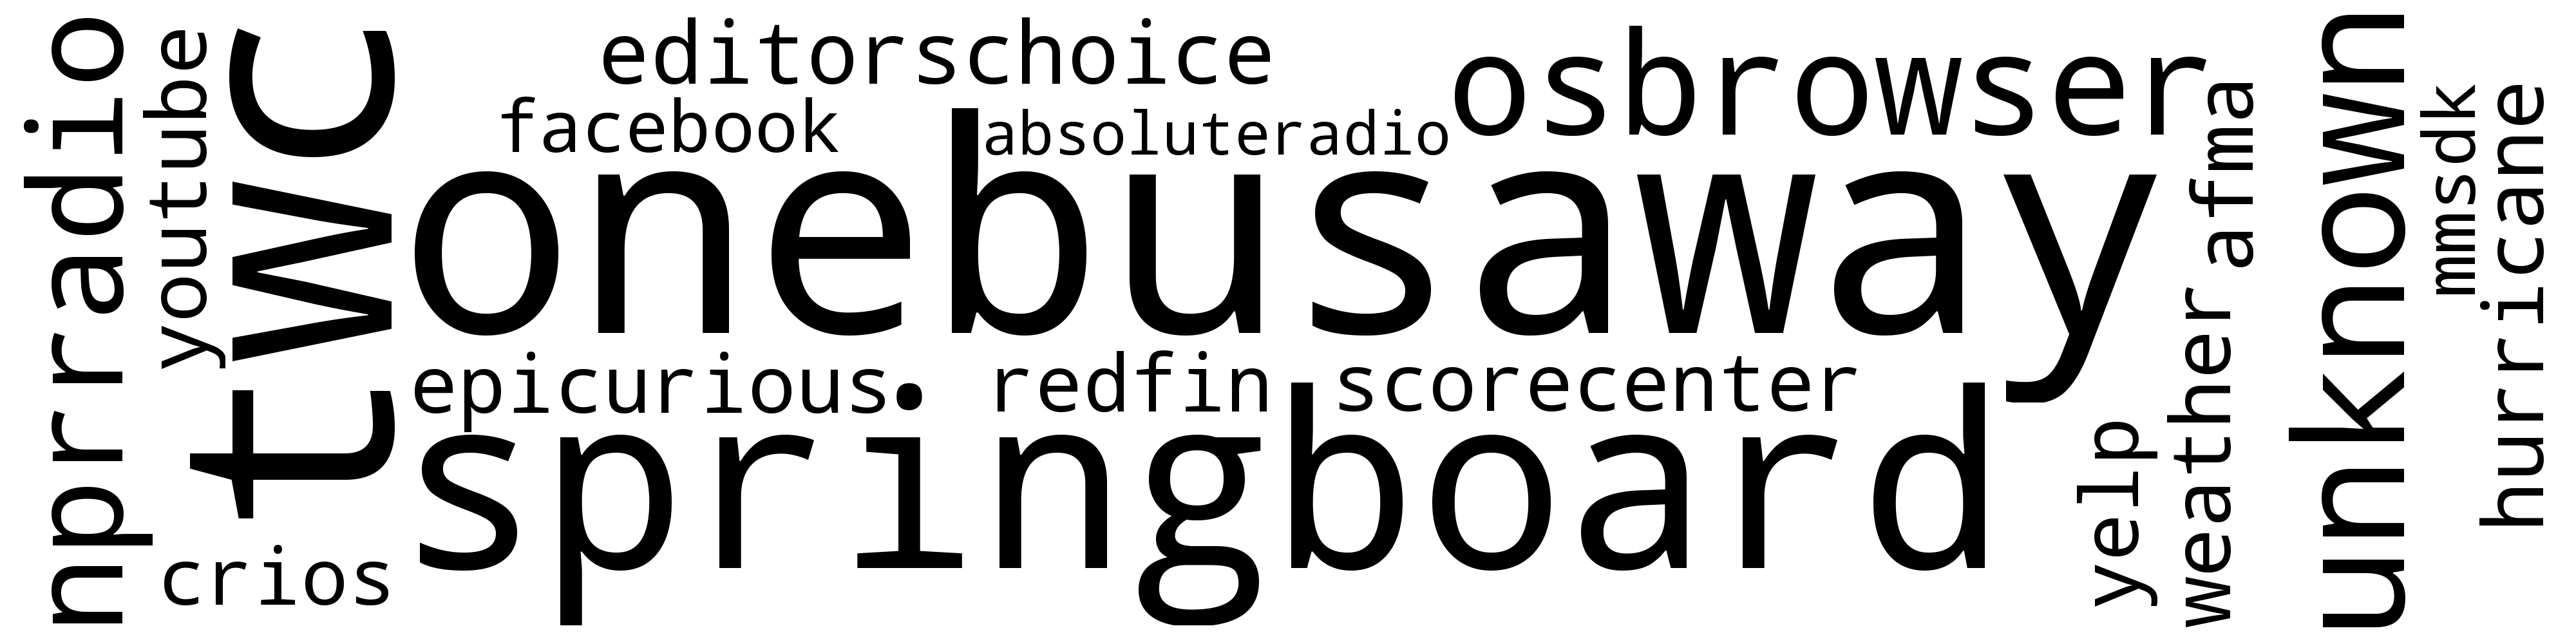
\includegraphics[width=\columnwidth]{figures/wordcloud_useragentsignature_location_image.png}}
%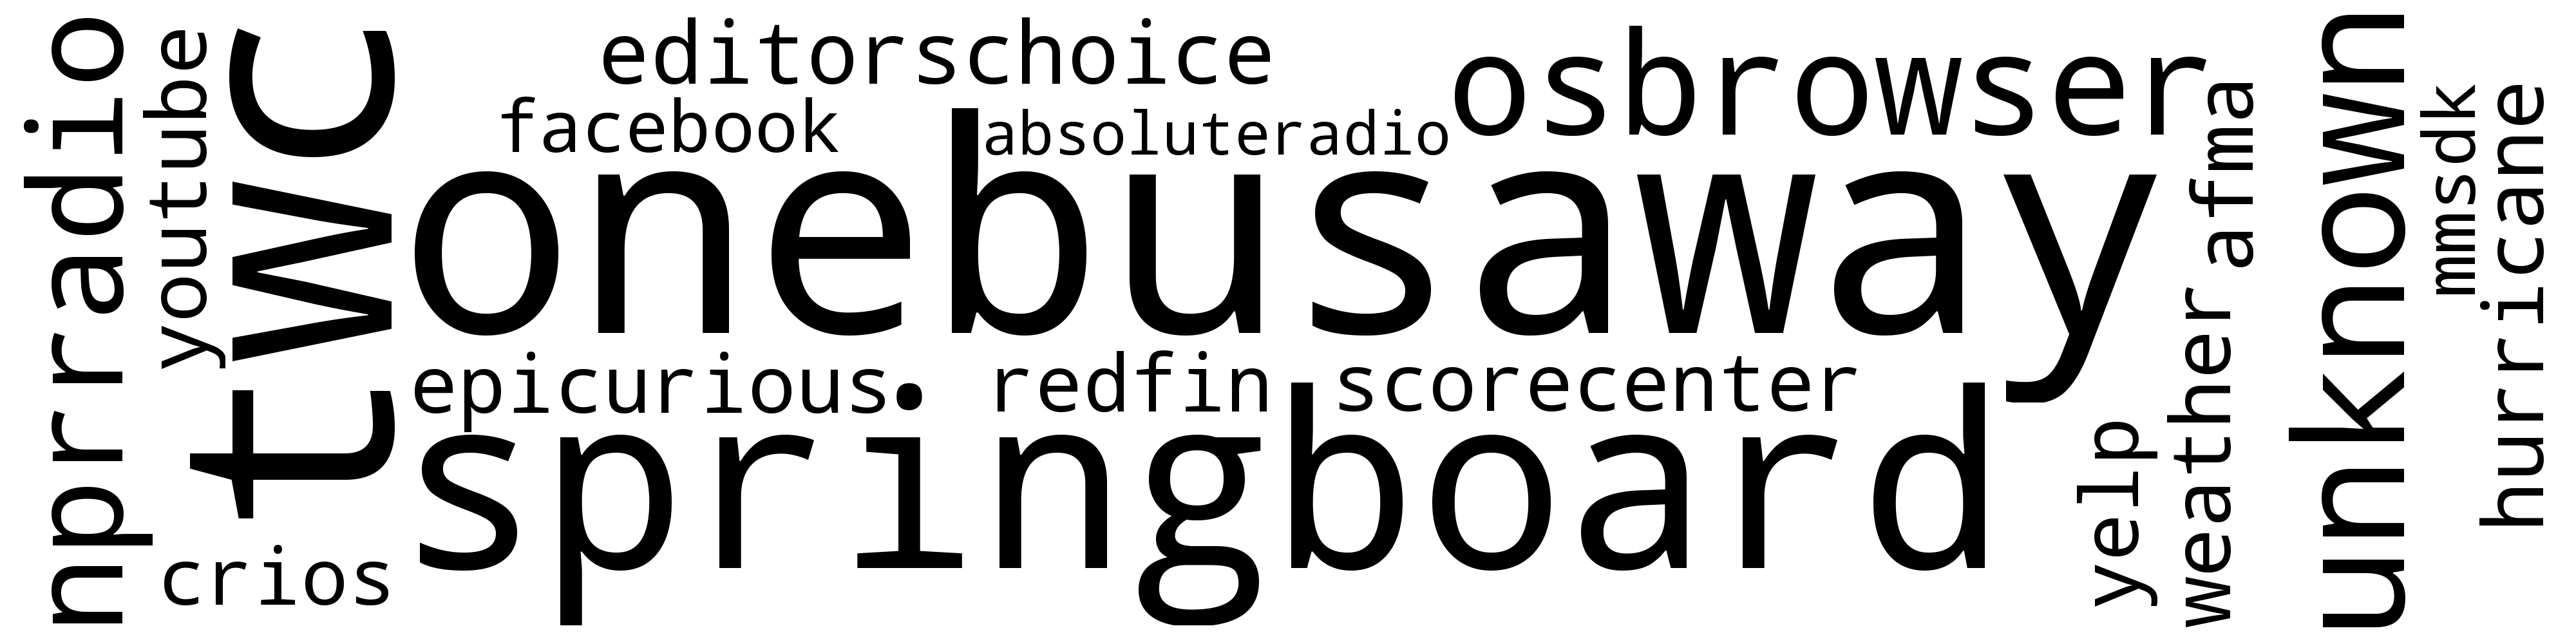
\includegraphics[width=\columnwidth]{figures/wordcloud_useragentsignature_location_image.png}
\newline
%\subfloat[Springboard \useragent strings leaking the device location.]{\label{fig:springboard}
%\begin{tabular}{|l|}
% \hline
% SpringBoard/50 CFNetwork/548.1.4 Darwin/11.0.0 \tabularnewline
% SpringBoard/50 CFNetwork/609 Darwin/13.0.0 \tabularnewline   
% SpringBoard/50 CFNetwork/609.1.4 Darwin/13.0.0 \tabularnewline
% \hline
% \end{tabular}}\newline
\subfloat[Frequency of leaks by \emph{SpringBoard}.]{\label{fig:springboard-wild} 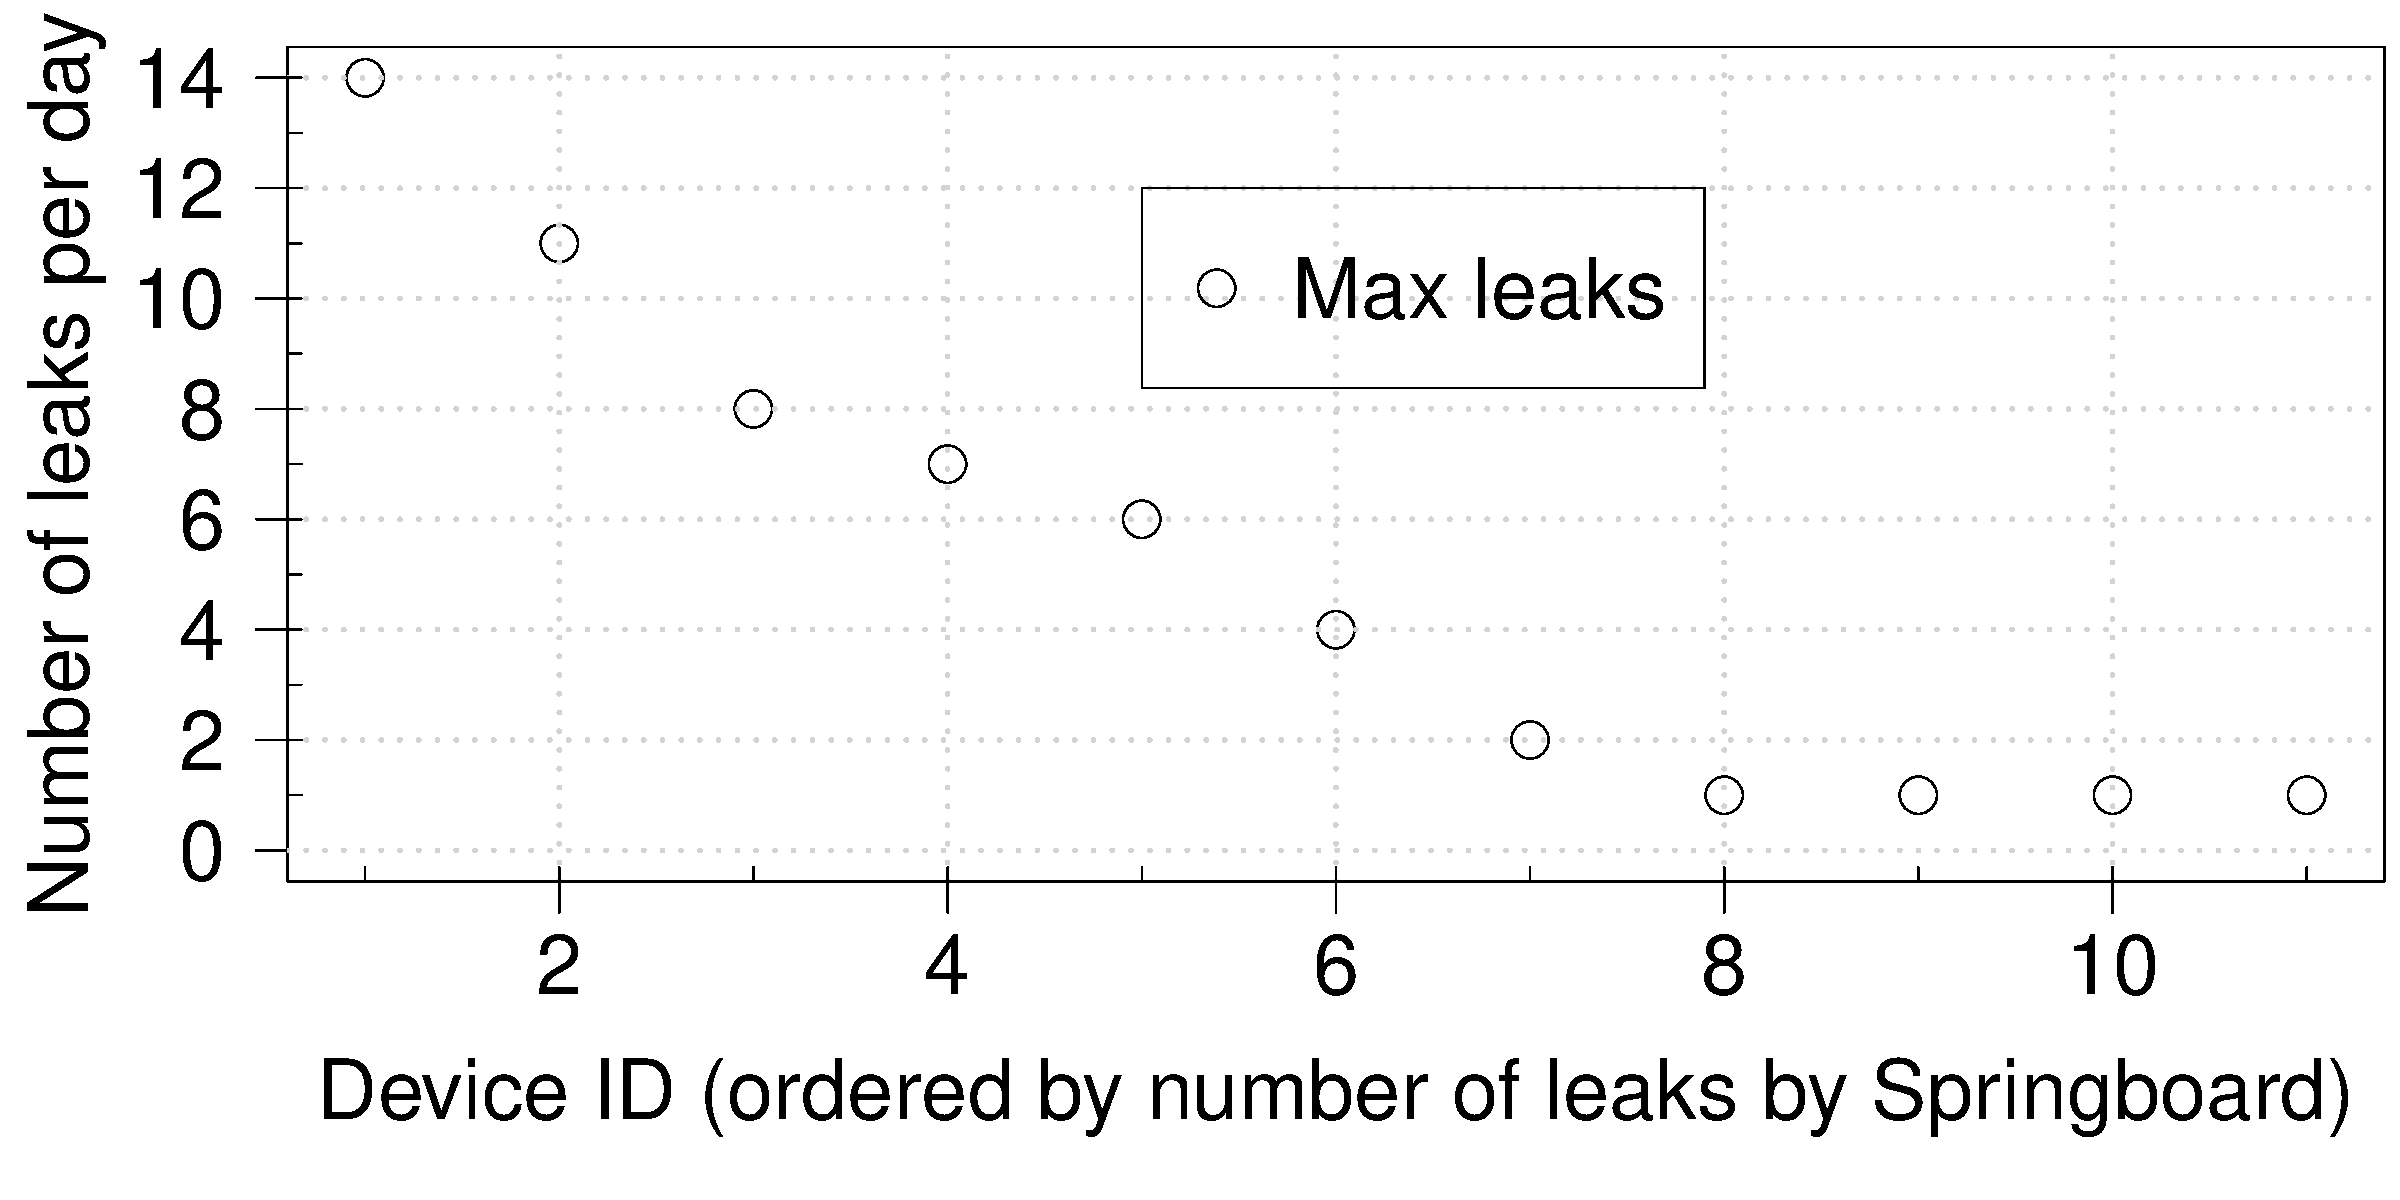
\includegraphics[width=0.9\columnwidth]{plots/piileaks_locclearspringboard.pdf}}
\caption{Apps that send the location information in the clear. \emph{The font size in the cloud represent the number of flows that sent the location information in the clear. We observe location leaks across different version of SpringBoard and from all the iPhones and the iPodtouch devices in the \mobWild dataset.}}
\label{fig:location-wordcloud}
\vspace{\postfigspace}
\end{figure}

In Figure~\ref{fig:location-wordcloud}, we present a \emph{word cloud} of
the apps that send the location information of the devices.
We observe that a bus service app (\emph{One Bus Away}), the
app that manages the iOS homescreen (\emph{SpringBoard}), and
weather apps (\emph{TWC}, \emph{Weather}, and \emph{Hurricane})
were responsible for more 78\% of the flows that sent the location
information in the clear. 
Further, \emph{SpringBoard} (the app responsible for managing the home screen of iOS devices) sends location information in the clear to fetch weather information from Yahoo servers. 
In Figure~\ref{fig:springboard-wild}, we observe that \emph{SpringBoard} leaked location information for 11 devices in the \mobWild dataset, a maximum of 14 leaks per day was observed for one device. 
We also observe that these devices include the iPodtouch device and all the iPhones in \mobWild, however, we do not observe such leaks for the iPad devices in the \mobWild dataset.  


In addition, we observe that the device ID and IMEI number of
devices in the \mobWild dataset are leaked in the clear.  Based on our
classification methodology, we observe that the IMEI number and device
ID is leaked by Web browsers; we do not observe any other app 
signature in non-browser flows leaking these IDs in the \mobWild dataset.  As in the case of
controlled experiments, A\&A sites are the most popular
destination for the IMEI number leaks.  Among the 16 sites that received 
the IMEI number in the clear, 10 are A\&A sites;
the rest of the sites includes sites for games, news, and manufacturer
updates.

\begin{table}
\centering
\begin{small}
\begin{tabular}{|p{0.35\columnwidth}|p{0.1\columnwidth}|p{0.15\columnwidth}|p{0.1\columnwidth}|}
\hline
\multirow{2}{*}{\bf Tracker} & \multicolumn{3}{c|}{\bf Number of devices tracked}\tabularnewline
\cline{2-4}
                      &  {\bf Total} & {\bf iOS} & {\bf Android} \tabularnewline
\hline
doubleclick.net       & 26 {\em(all)} & 15 {\em(all)} & 11 {\em(all)} \tabularnewline
\hline
google-analytics.com  & 26 {\em(all)} & 15 {\em(all)}  & 11 {\em(all)} \tabularnewline
\hline
googlesyndication.com & 22 & 12 & 10 \tabularnewline
\hline
admob.com             & 21 & 11 & 10 \tabularnewline
\hline
scorecardresearch.com &  21 & 11 & 10 \tabularnewline
\hline
\end{tabular}
\end{small}
\caption{The top 5 ads and analytics sites that were contacted by the devices in our dataset.
\emph{The sites, doubleclick.net and google-analytics.com, were contacted by all the 26 devices in} \mobWild.}
\label{tab:top-trackers}
\end{table}

In Table~\ref{tab:top-trackers}, we present the number of devices in the \mobWild dataset that contact the most popular A\&A sites, an activity that is receiving considerable attention~\cite{roesner:webtrackers,leontiadis:mobileads,vallina-rod:ads}.
We observe that all the devices in the \mobWild dataset contacted doubleclick.com, an ad site, and google-analytics.com, a tracking site. 
Further, 66.12\% of the ads and analytics traffic volume in the \mobWild dataset was from browsers, 6.46\% of the
traffic contained a blank user-agent field, and 4.8\% of the traffic contained a signature of \emph{Google-Analytics} library.
The rest of the traffic contained signatures of other apps such as Facebook, Pandora, and YouTube.

Given the extensive nature of tracking over mobile devices, we developed a tool, \emph{ConVis} that allows users to visualize their devices' tracking, and the apps that facilitate this tracking, with the help of a web-based interfaces similar to that of Mozilla Collusion~\cite{collusion}. \emph{ConVis} provides a visual interface that allows 
 users to specify block lists for connections based on (app, 3rd party) tuples. A demo of our tool is 
 located at \url{http://goo.gl/A17h9}. 
%\tbd{A demo of this can be found at ...}
%\tbd{Add some comment about ConVis (Nick's work), say that it's another 
%contribution in that it helps average users visualize their tracking and PII, 
%and that we make it available to participating users, and the URL for the 
%demo is at location X.}



%%% Local Variables: 
%%% mode: latex
%%% TeX-master: "main"
%%% End: 

%       getjar.com     & - S & - S \tabularnewline
%       aarki.net      & - S & - - \tabularnewline
%       chartboost.com & - S & - S \tabularnewline
%       *pocketexchange&   S &   S \tabularnewline
%       *vserv.mobi    & - - & C   \tabularnewline
%       *groupon.com   &     &   S
%       *flurry.com    &     &   S
%       *bankofamerica &     &   S
%       *google.com    & - - & - S

%\section{MISC}

% \begin{figure}
% \centering
% \includegraphics[width=\columnwidth]{plots/ads_wild_gatracking.pdf}
% \caption{Number of devices tracked by Google-Analytics. \emph{We observe that devices }}
% \label{fig:tracking-analytics}
% \end{figure}

% \begin{figure}
% \centering
% \includegraphics[width=\columnwidth]{plots/ads_wild_usertracking.pdf}
% \caption{Number of sites that track a user. \emph{We observe that devices }}
% \label{fig:tracking-analytics}
% \end{figure}

% \begin{figure}
% \centering
% \includegraphics[width=\columnwidth]{plots/ads_wild_sitescontacted.pdf}
% \caption{Number of visits to A\&A sites per device. \emph{The error bars indicate the 25$^{th}$ and 75$^{th}$ percentiles. Each visit is a potential tracking visit.}}
% \label{fig:tracking-analytics}
% \end{figure}

% \begin{table}    
%     \centering
%     \begin{small}
%     \begin{tabular}{|l|c|c|}
%        \hline
%        {\bf Host}&{\bf IMEI}&{\bf Device ID}\tabularnewline
%        \hline              
%        tapjoyads.com  & Y & - \tabularnewline
%        zynga.com      & Y & - \tabularnewline
%        iheart.com     & Y & Y \tabularnewline
%        google.com     & - & Y \tabularnewline
%        flurry.com     & - & Y \tabularnewline
%        \hline
%     \end{tabular}
%     \end{small}
%     \caption{Hosts to which the IMEI or Device ID was sent in the clear and over HTTPS. \emph{The value Y for a column implies that data was sent over HTTP and HTTPS. We order these hosts based on the number of flows that sent the IMEI number in the clear and over HTTPS.}}
%     \label{tab:pii-leakage-sites}
% \end{table}

%Moreover, we observe that 4\% of the flows
%sent the location information to ads and analytics sites; the rest of the
%flows being from apps including browsers, the Facebook app, and angry birds. 
% more than
%80\% of \emph{ad-flows} leaking location information did not include
%an application signature in the user-agent field, 
%Similarly, from the device of one of the authors of the paper, we observed that the latest three versions YahooMail application, up to the time of the measurements, leaked the user's email address in the clear.


%\tbd{This should come before 
%We first identify A\&A flows using the publicly available database of~\cite{YoyoAds}; we augment this list of domains using recent research on mobile ads~\cite{hornyack:appfence, leontiadis:mobileads}.
%Based on this classification, we observe that the ads and analytics traffic was responsible for up to 6\% of the traffic by volume per device, an observation in line to the one made by Vallina-Rodriguez~\etal~\cite{vallina-rod:ads}}.

%\subsection{Ads and Analytics in the Wild}

% \tbd{focusing on ads and analytics is just what you did in the
%   previous paragraph. What is new or different in this one.}
% We now focus our attention on the extent to which devices in the
% \mobWild dataset contact ads and analytics (A\&A) sites, an activity
% that is receiving considerable
% attention~\cite{roesner:webtrackers,leontiadis:mobileads,vallina-rod:ads}.
% Using our classification based on the \httphost, we observe that the
% ads and analytics traffic was responsible for up to 6\% of the traffic
% by volume per device, an observation in line with the one made by
% Vallina-Rodriguez~\etal~\cite{vallina-rod:ads}.  Rather that focusing
% on the traffic volume we focus on the extent to which these sites are
% able to track the users in the dataset and the applications that
% facilitate this tracking.
%\tbd{This must come before Furthermore, we observed that 7\% of the traffic contained the Google-Analytics in the signature field; this signature was observed even in the flows for users that did not have the Google Analytics application installed on the device. Mention that we will wrongly classify the flows from Google Analytics app as ads and analytics traffic} 

